% !TeX spellcheck = de_DE

\documentclass[12pt,a4paper,parskip=half]{scrreprt}

\usepackage[english]{babel}
\usepackage[utf8]{inputenc}
\usepackage{acronym}
\usepackage{graphicx}
\usepackage[below]{placeins}
\usepackage{url}
\usepackage{hyperref}
\usepackage{tabularx}
\usepackage{booktabs}
\usepackage{textcomp}
\usepackage{caption}

% font coloring
\usepackage{xcolor}
% for tables
\usepackage{multirow}

\newcommand{\source}[1]{\caption*{Source: {#1}} }

\title{Bericht Praxisphase I}
\author{Sebastian Wallat}
\date{\today}

\clubpenalty = 10000 % schliesst Schusterjungen aus
\widowpenalty = 10000 % schliesst Hurenkinder aus

\graphicspath{{./images/}}

\begin{document}

\begin{titlepage}
	
	\centering
	
%%	\ifcsempty{iodhbwm@institute@logo}{%
		
%%		
\includegraphics[height=1.5cm]{dhbw-logo}
		
	{%
		
		\begin{minipage}[c]{.25\textwidth}
			
			
\includegraphics[width=\textwidth, height = 2cm]{dhbw-logo}
			
		\end{minipage}
		\begin{minipage}[c]{0.46\textwidth}
			
			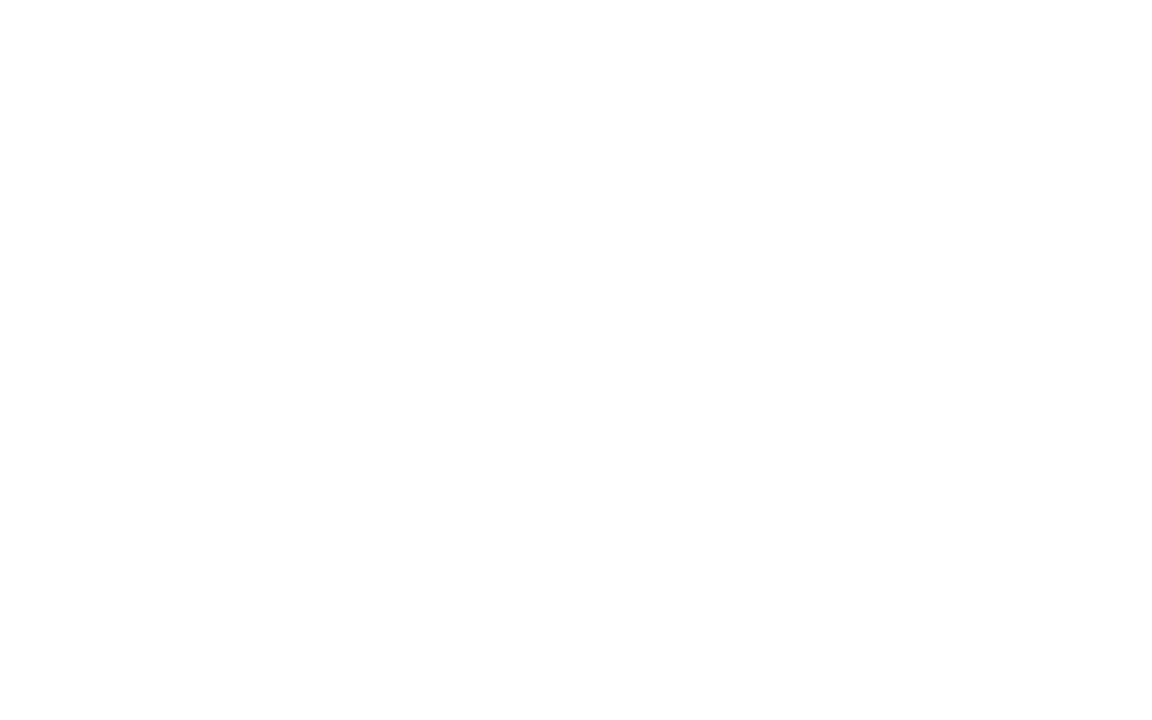
\includegraphics[width=\textwidth]{empty}
			
		\end{minipage}
		\begin{minipage}[c]{.25\textwidth}
			
			\raggedleft
			
			
\includegraphics[width=\textwidth, height =2cm, keepaspectratio]{dlr-logo}
			
		\end{minipage}
		
	}
	
	
	
	\bigskip
	
	
	
	\Large\textsc{Hausarbeit}
	
	
	
	\normalsize
	
	des Studiengangs Informationstechnik\par
	
	der Dualen Hochschule Baden-Württemberg Mannheim
	
	
	
	\rule{\textwidth}{.5mm}\bigskip
	
	
	
	\textsc{\large Sicherheit und Fehlermodelle von verteilten Systemen}	
	
	
	\rule{\textwidth}{.5mm}
	
	
	
	\vfill
	
	
	
	\par
	
	{\bfseries\large Julian Fuchs, Marius Bröcker, Sebastian Wallat}\par
	
	\today
	
	
	
	\vfill
	
	
	
	\small{%
		
		\begin{tabularx}{\textwidth}{@{}lX@{}}
			
			\toprule
			
			
			Bearbeitungszeitraum: & 24.10.2020-27.11.2020\\
			
			Matrikelnummer, Kurs: & 1708267, TINF18-IT1\\
			
			Vorlesung: & Verteilte Systeme \\
			
		\end{tabularx}
		
	}
	
	\cleardoublepage
	
\end{titlepage}


\newpage
\pagenumbering{Roman}

\chapter*{Eidesstattliche Erklärung}
%%\thispagestyle{empty}
\vspace{50pt}
Wir versichern hiermit, dass wir diese Hausarbeit mit dem Thema: ''Sicherheit und Fehlermodelle von verteilten Systemen'' selbständig verfasst und keine anderen als die angegebenen Quellen und Hilfsmittel benutzt haben.
\\
\\

\vfill
\noindent\rule{5cm}{.4pt}\hfill\rule{5cm}{.4pt}\par
\noindent Datum, Ort \hfill Unterschrift 

\newpage
\thispagestyle{empty}
\chapter*{Zusammenfassung}

Thema
\\
\bigskip

\tableofcontents
\addtocontents{toc}{}

\listoffigures
\addcontentsline{toc}{chapter}{Abbildungsverzeichnis} 
%%\thispagestyle{empty}

\newpage
\chapter*{Abkürzungsverzeichnis}
\addcontentsline{toc}{chapter}{Abkürzungsverzeichnis}
%%\thispagestyle{empty}
\begin{acronym}[HTTP]
	\acro{DLR}{\textbf{D}eutsches Zentrum für \textbf{L}uft- und \textbf{R}aumfahrt}
\end{acronym}

\pagenumbering{arabic}

\chapter{Einführung}


\chapter{Sicherheit}


\section{Schutzziele}


\section{Angriffsvektoren}


\section{Schutzmaßnahmen}


\subsection{Verschlüsselung}


\subsection{Authentisierung}


\subsection{Autorisierung}


\chapter{Fehlermodelle}
Sowohl System externe als auch interne Fehlerereignisse und Störungen können die Stabilität und Verfügbarkeit eines Systems komprimieren. Zu externen Störungen lassen sich unter anderem Natureinflüsse (wie Stromausfälle) oder gezielte Attacken auf die zuvor definierten Schutzziele zählen. Interne Störungen umfassen Hardware-Probleme (wie Festplatten-Ausfälle) und Software-Probleme zählen. Verteilte Systeme sind dabei durch den physikalisch getrennten Aufbau weniger Anfällig für Komplettausfälle. In der Regel sind bei Störungen einzelne Komponenten oder Teilsysteme betroffen. Gleichzeitig kann es durch den komplexeren Aufbau zu regelmäßigeren Ausfällen kommen (wie durch Wartungsarbeiten) und Fehler in einer Komponente könnten sich auf andere übertragen. Ein wichtiger Teil eines verteilten Systems umfasst damit auch die Vorbeugung von und den Umgang mit Ausfällen von Teilsystemen.

\section{Anforderungen}
%Ziel: Fehlertoleranz\\
%- Verfügbarkeit\\
%- Zuverlässigkeit\\
%- Funktionssicherheit\\
%- Wartbarkeit\\
Ausfälle und Störungen eines Teilsystems gänzlich vorzubeugen ist sehr schwer -- wenn nicht unmöglich. Ein zentrales Ziel muss daher sein, ein verteilten Systems so aufzubauen, dass es eine gewissen Fehlertoleranz besitzt. Die Fehlertoleranz beschreibt die Eigenschaft eines Systems bei Störungen eine korrekte Funktionsweise aufrecht zuhalten, ohne schwerwiegende Leistungsminderungen einbüßen zu müssen. \\
Um dieses Ziel gewährleisten zu können, muss ein verteiltes System mehrere Anforderungen erfüllen. Zu diesen zählen die Fähigkeiten des Systems einen Fehler zu erkennen, eine konstante Verfügbarkeit dieses, eine gewisse Zuverlässigkeit und Funktionssicherheit des Systems. Zuletzt spielt die Wartbarkeit eines solchen Systems eine wichtige Rolle. Die Anforderungen sind in \autoref{tbl:fehlertoleranz} erneut aufgeführt und erläutert. 
\begin{table}[h]
	\centering
%	\resizebox{\textwidth}{!}{%
	\begin{tabular}[h]{ll}
		\toprule
		Anforderung 		& Beschreibung \\
		\midrule
		Fehlererkennung		& Um fehlertolerant zu sein, muss ein System \\
							& Ausfälle erkennen und auf diese reagieren \\
							& können \vspace{4pt} \\
		Verfügbarkeit 		& Das System und dessen Dienste sind stets ver-\\
							& fügbar und erreichbar \vspace{4pt}\\
		Zuverlässigkeit		& Ein System wird durchgehend fehlerfrei ausge-\\
							& führt \vspace{4pt}\\
		Funktionssicherheit	& Störungen im System komprimieren nicht die \\
							& Sicherheit von Daten oder führen nicht zu un- \\
							& gewollten Aktionen und Ergebnissen \vspace{4pt}\\
		Wartbarkeit 		& Beschreibt den Aufwand der Wartung eines\\
							& Systems 
							\\			
		\bottomrule
	\end{tabular}
%	}
	\captionsetup{font = small}
	\caption{Anforderungen an ein System, um fehlertolerant zu sein \\
		\textcolor{red}{(soll Tabelle bestehen bleiben oder in Klartext umgewandelt werden?)}}
	\label{tbl:fehlertoleranz}
\end{table}

\section{Arten von Fehlern und Störungen}
Auftretende Fehler und Störung lassen sich vorab in drei Kategorien einteilen. \textit{Transiente}, sich \textit{wiederholende} und \textit{permanente} Fehler.\\
\textit{Transiente Fehler} beschreiben dabei einmalig auftretende Störungen. Diese sind oft schwer vorherzusagen und folglich schwer zu bekämpfen, da diese oft unter einmaligen oder sehr bestimmten Voraussetzungen eintreten.\\
\textit{Wiederholende Fehler} treten periodisch oder bei bestimmten Voraussetzungen auf....\\
\textit{Permanente Fehler} beschreiben andauernde Störungen...\\


%- Vorübergehend\\
%- Wiederkehrend\\
%- Permanent\\
~\\
- Absturz\\
- Dienstausfall\\
- Zeitbedingter Ausfall\\
- Ausfall korrekter Antwort\\
- Byzantinischer oder zufälliger Ausfall
\\
- Ausfall von Client\\
- Kommunikationssystem\\
- (Teil-)System\\

\section{Fehlerbehebung}
- wichtig: Redundanz\\
- Replikation von Prozessen etc.\\



\newpage

\nocite{*}
\thispagestyle{headings}

\bibliographystyle{IEEEtr}
\bibliography{bibo} 


\end{document}